\begin{figure}[!h]
    \centering
    \begin{subfigure}{.5\textwidth}
      \centering
      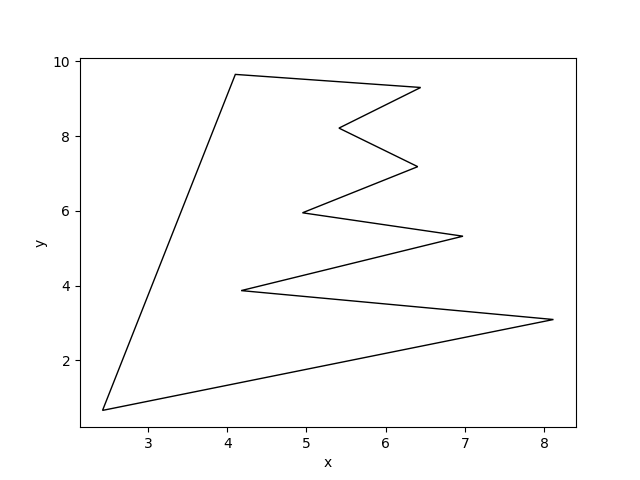
\includegraphics[width=.9\linewidth]{polygon_5.png}
      \caption*{Rys. 1: Pięciokąt.}
      \label{fig:sub1}
    \end{subfigure}%
    \begin{subfigure}{.5\textwidth}
      \centering
      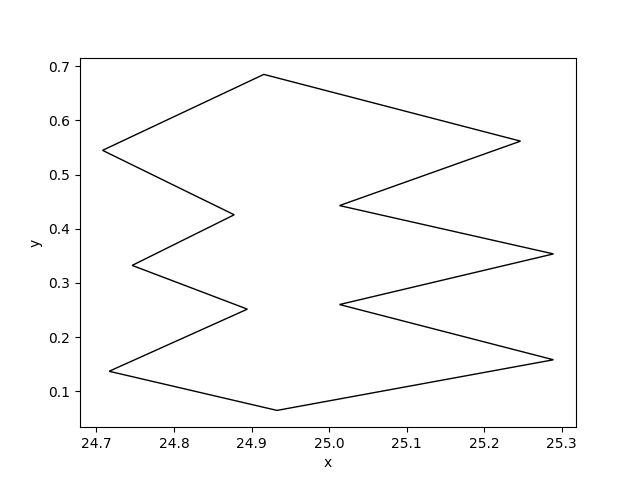
\includegraphics[width=.9\linewidth]{christmas_tree.png}
      \caption*{Rys. 2: Choinka.}
      \label{fig:sub2}
    \end{subfigure}
    \label{fig:test}
    \end{figure}

\newpage

    \begin{figure}[!h]
    \centering
    \begin{minipage}{.5\textwidth}
      \centering
      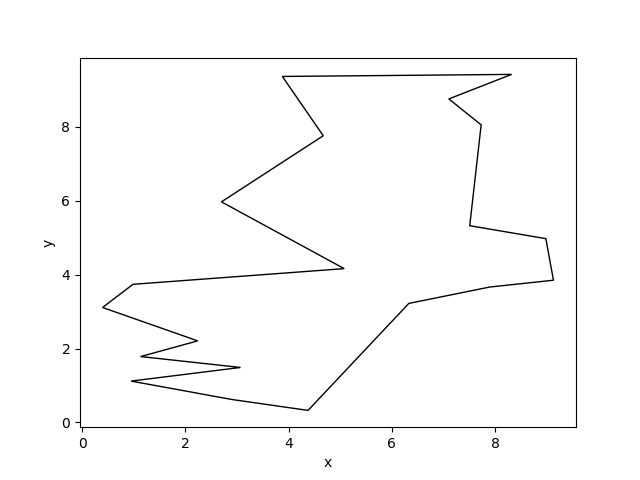
\includegraphics[width=.9\linewidth]{polygon_weird.png}
      \caption*{Rys. 3: Wielokąt 1.}
      \label{fig:test1}
    \end{minipage}%
    \begin{minipage}{.5\textwidth}
      \centering
      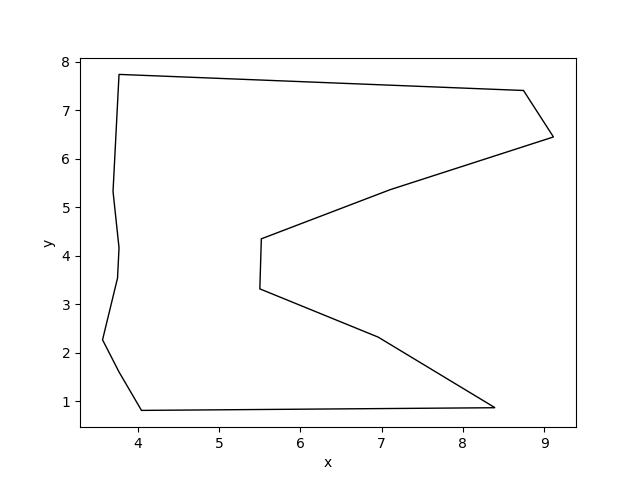
\includegraphics[width=.9\linewidth]{polygon_weird_2.png}
      \caption*{Rys. 4: Wielokąt 2.}
      \label{fig:test2}
    \end{minipage}
    \end{figure}
    \begin{figure}[!h]
        \centering
        \begin{minipage}{.5\textwidth}
          \centering
          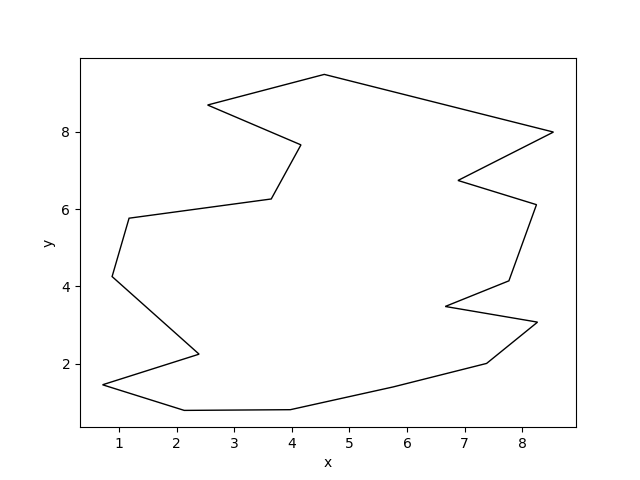
\includegraphics[width=.9\linewidth]{polygon_weird_3.png}
          \caption*{Rys. 5: Wielokąt 3.}
          \label{fig:test1}
        \end{minipage}%
        \begin{minipage}{.5\textwidth}
          \centering
          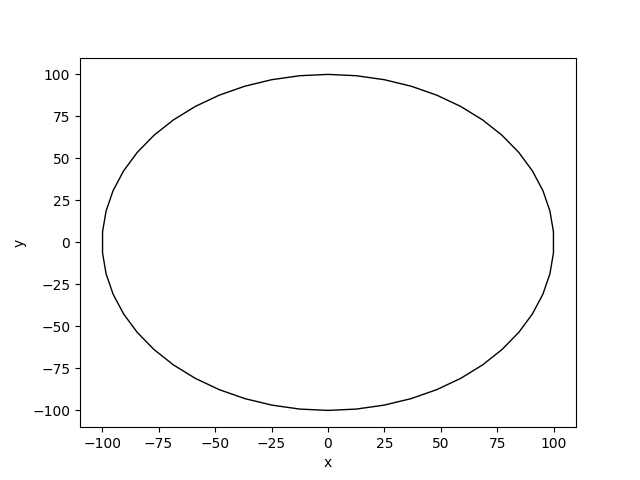
\includegraphics[width=.9\linewidth]{polygon_50.png}
          \caption*{Rys. 6: 50-kąt foremny.}
          \label{fig:test2}
        \end{minipage}
        \end{figure}